\documentclass[conference]{IEEEtran}
\usepackage{color}
\usepackage{float}
\usepackage{graphicx}
\usepackage{amsmath}
\usepackage{listings}



\definecolor{mygreen}{RGB}{28,172,0} % color values Red, Green, Blue
\definecolor{mylilas}{RGB}{170,55,241}
\lstset{language=Matlab,%
    %basicstyle=\color{red},
    breaklines=true,%
    }
    
  \DeclareGraphicsExtensions{.jpg}

\begin{document}

\title{IMPLEMENTING K-MEANS CLUSTERING}

\author{\IEEEauthorblockN{Tahjib Hassan Rhythm}
\IEEEauthorblockA{Department of Computer Science and Engineering\\
Ahsanullah University of Science and Technology\\
Tejgao, Dhaka, Bangladesh}}

\maketitle
\begin{abstract}
This experiment is to understand one of the very popular clustering algorithm known as K-Means clustering algorithm. This is an unsupervised learning method which means the class label is unknown here. But to measure the performance of the algorithm we need to know the ground truth. Here in this experiment we will use cluster purity as performance measure of the classifier. Here we use the dataset that has 150 data with four dimension each. We will cluster the whole dataset into three cluster here, so in our experiment k=3. 
\end{abstract}
\IEEEpeerreviewmaketitle

\section{INTRODUCTION}
K-means is one of the simplest unsupervised learning algorithms that solve the well known clustering problem. The procedure follows a simple and easy way to classify a given data set through a certain number of clusters (assume k clusters) fixed a priority. The main idea is to define k centroids, one for each cluster. These centroids shoud be placed in a cunning way because of different location causes different result. So, the better choice is to place them as much as possible far away from each other.

\begin{figure}[H]
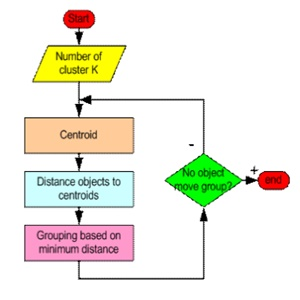
\includegraphics[width=\linewidth]{fc.jpg}
\caption{Flow Chart of K-Means Clustering}
\end{figure}

1. Choosing the initial centroids . \\
2. Determine the distance of each object to the centroids.\\
3. Group the object based on minimum distance.\\

The next step is to take each point belonging to a given data set and associate it to the nearest centroid. When no point is pending, the first step is completed and an early groupage is done. At this point we need to re-calculate k new centroids as barycenters of the clusters resulting from the previous step. After we have these k new centroids, a new binding has to be done between the same data set points and the nearest new centroid. A loop has been generated. As a result of this loop we may notice that the k centroids change their location step by step until no more changes are done. In other words centroids do not move any more. Flow of works is:

1. Determine the centroid coordinate \\
2. Calculating the distance matrix \\
3. Calculating new centroids until centroids change\\

\section{IMPLEMENTATION}

\subsection{Choosing the initial centroids}

Since in this experiment we choose to cluster the whole dataset in three cluster we have to choose three centroids. At first we choose it randomly but the centroid should be as far as possible so we fixed the range. The first centroid will be between 0 and 50 the second one will be between 50 and 100 and the third one will be between 101 and 150.

\subsection{Calculating the distance matrix}

Here in this experiment we calculate the Euclidian distance between the sample points and centroid in a 3 x 150 matrix. After that this distance matrix will be used to assign groups to each column of the distance matrix. Here we have 150 column so we will get 150 one in the group matrix but in different row. In which row it will be determined by the minimum distance stored in the distance matrix.  After assigning the group now we have to count that how many sample are in each group/cluster. Then we will calculate the new centroids for the next iteration. 

\subsection{Calculating new centroids until centroids change}

The new centroid will be all the data samples average which corresponding row has a 1 in the group matrix. Thus we will get new set of centroid. After that the whole procedure will continue until 20 times of the time each group has the same number of samples.  In our experiment the result is 50 61 39 most of the time. It will change sometimes cause the initial centroid are chosen randomly. So it is possible to get slight different output but the difference won’t be very high.

\subsection{Plotting different clusters}

After the iteration where the cluster coordinates do not change we simply have to plot the cluster having samples of its own. We have done this in the following figure:

\begin{figure}[H]
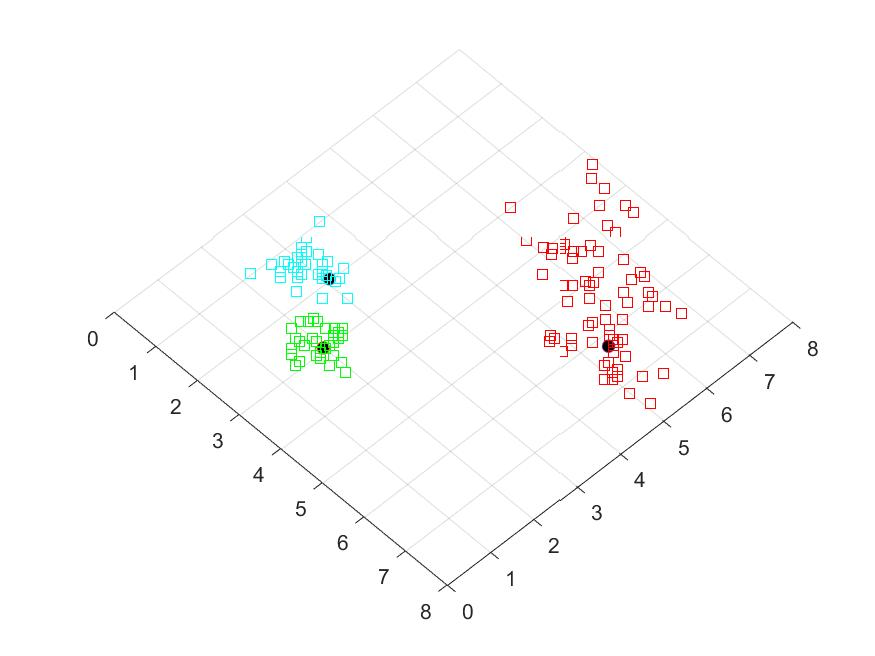
\includegraphics[width=\linewidth]{res.jpg}
\caption{Clustering Groups}
\end{figure}

\section{RESULT ANALYSIS}
From the figure -2, we can see that we have found  three groups colored red, green, and cyan from a randomly chosen centroids and tuning it to perfection until we found the identical set of matrix to represent the clusters. \\

One basic metric to measure how "good" the clustering in comparison to known class labels is called purity.\\

To compute purity, each cluster is assigned to the class which is most frequent in the cluster, and then the accuracy of this assignment is measured by counting the number of correctly assigned documents and dividing by N. where N is the total number of samples. In our experiment the 150 dataset is actually divided into 50 50 and 50 members. Our result is 50 61 39. So for the first cluster the cluster purity is 50/50 =1 For the second cluster it is 61/50 = 1.22 For the third cluster it it 39/50 = 0.78 So the total purity is (1+1.22+0.78) = 3 \\
 
So what does this tell us? A cluster is considered to be "pure" if it has a purity of 1 since that indicates that all of the instances in that cluster are of the same label. This means our original label classification was pretty good and that our Kmeans did a pretty good job. The "best" purity score for an entire data set would be equal to the original K-number of clusters since that would imply that every cluster has an individual purity score of 1. 

\section{MATLAB CODE}
\begin{lstlisting}
x=zeros(150,4);
myfile=fopen('irisdataset.txt','r');
x=fscanf(myfile,'%f\t%f\t%f\t%f',size(x));
figure,hold on;

grid on;
hold off;

randomRow = randi([1,150]);
c1 = [x(randomRow,1) x(randomRow,2) x(randomRow,2) x(randomRow,4)];

randomRow = randi([1,150]);
c2 = [x(randomRow,1) x(randomRow,2) x(randomRow,2) x(randomRow,4)];

randomRow = randi([1,150]);
c3 = [x(randomRow,1) x(randomRow,2) x(randomRow,2) x(randomRow,4)];

d1 = zeros(1,150);
d2 = d1;
d3 = d1;
for i = 1:150
    d1(1,i) = sqrt((c1(:,1) - x(i,1)) * (c1(:,1) - x(i,1)) + (c1(:,2) - x(i,2)) * (c1(:,2) - x(i,2)) + (c1(:,1) - x(i,3)) * (c1(:,1) - x(i,3)) + (c1(:,2) - x(i,4)) * (c1(:,2) - x(i,4))) ;
    d2(1,i) = sqrt((c2(:,1) - x(i,1)) * (c2(:,1) - x(i,1)) + (c2(:,2) - x(i,2)) * (c2(:,2) - x(i,2)) + (c2(:,1) - x(i,3)) * (c2(:,1) - x(i,3)) + (c2(:,2) - x(i,4)) * (c2(:,2) - x(i,4))) ;
    d3(1,i) = sqrt((c3(:,1) - x(i,1)) * (c3(:,1) - x(i,1)) + (c3(:,2) - x(i,2)) * (c3(:,2) - x(i,2)) + (c3(:,1) - x(i,3)) * (c3(:,1) - x(i,3)) + (c3(:,2) - x(i,4)) * (c3(:,2) - x(i,4))) ;
end
d = [d1; d2; d3];
g = d;
for j = 1:150
    min = 50000;
    index = 0;
    for i = 1:3
        if(d(i,j) < min)
            min = d(i,j);
            index = i;
        end
    end
    for i = 1:3
         g(i,j) = 0;
    end
    g(index,j) = 1;
end

%CLUSTERING LOOP
for w=1:20 
tempG = g;

for j = 1:150
    for i = 1:3
        if(g(i,j)==1 && i==1)
          newX1 = (x(j,1) + c1(1,1))/2;
          newX2 = (x(j,2) + c1(1,2))/2;
          newX3 = (x(j,3) + c1(1,3))/2;
          newX4 = (x(j,4) + c1(1,4))/2;
          c1 = [newX1 newX2 newX3 newX4];
        elseif(g(i,j)==1 && i==2)
          newX1 = (x(j,1) + c2(1,1))/2;
          newX2 = (x(j,2) + c2(1,2))/2;
          newX3 = (x(j,3) + c2(1,3))/2;
          newX4 = (x(j,4) + c2(1,4))/2;
          c2 = [newX1 newX2 newX3 newX4];
        elseif(g(i,j)==1 && i==3)
          newX1 = (x(j,1) + c3(1,1))/2;
          newX2 = (x(j,2) + c3(1,2))/2;
          newX3 = (x(j,3) + c3(1,3))/2;
          newX4 = (x(j,4) + c3(1,4))/2;
          c3 = [newX1 newX2 newX3 newX4];
        end
    end
end
d1 = zeros(1,150);
d2 = d1;
d3 = d1;
for i = 1:150
    d1(1,i) = sqrt((c1(:,1) - x(i,1)) * (c1(:,1) - x(i,1)) + (c1(:,2) - x(i,2)) * (c1(:,2) - x(i,2)) + (c1(:,1) - x(i,3)) * (c1(:,1) - x(i,3)) + (c1(:,2) - x(i,4)) * (c1(:,2) - x(i,4))) ;
    d2(1,i) = sqrt((c2(:,1) - x(i,1)) * (c2(:,1) - x(i,1)) + (c2(:,2) - x(i,2)) * (c2(:,2) - x(i,2)) + (c2(:,1) - x(i,3)) * (c2(:,1) - x(i,3)) + (c2(:,2) - x(i,4)) * (c2(:,2) - x(i,4))) ;
    d3(1,i) = sqrt((c3(:,1) - x(i,1)) * (c3(:,1) - x(i,1)) + (c3(:,2) - x(i,2)) * (c3(:,2) - x(i,2)) + (c3(:,1) - x(i,3)) * (c3(:,1) - x(i,3)) + (c3(:,2) - x(i,4)) * (c3(:,2) - x(i,4))) ;
end
d = [d1; d2; d3];
g = d;
for j = 1:150
    min = 50000;
    index = 0;
    for i = 1:3
        if(d(i,j) < min)
            min = d(i,j);
            index = i;
        end
    end
    for i = 1:3
         g(i,j) = 0;
    end
    g(index,j) = 1;
end

if(tempG==g)
    break;
else 
    tempG=g;
end
end
display(w);

hold on;
plot(c1(:,1), c1(:,2),c1(:,3),c1(:,4), 'o', 'MarkerFaceColor', 'black');
hold off;
hold on;
plot(c2(:,1), c2(:,2),c2(:,3),c2(:,4), 'o', 'MarkerFaceColor', 'black');
hold off;
hold on;
plot(c3(:,1), c3(:,2),c3(:,3),c3(:,4), 'o', 'MarkerFaceColor', 'black');
hold off;

counterG1=0;
counterG2=0;
counterG3=0;
for j = 1:150
    for i = 1:3
        if(g(i,j)==1 && i==1)
          counterG1=counterG1+1;
          hold on; plot(x(j,1), x(j,2),x(j,3),x(j,4), 'gs'); hold off;
        elseif(g(i,j)==1 && i==2)
          counterG2=counterG2+1;
          hold on; plot(x(j,1), x(j,2),x(j,3),x(j,4), 'rs'); hold off;
        elseif(g(i,j)==1 && i==3)
          counterG3=counterG3+1;
          hold on; plot(x(j,1), x(j,2),x(j,3),x(j,4), 'cs'); hold off;
        end
    end
end
display(counterG1);
display(counterG2);
display(counterG3);
\end{lstlisting}
\section{CONCLUSION}

In this experiment we explore the K-means clustering algorithm. This is a very popular and widely used clustering technique. In this algorithm we need to know the ground truth if we want to measure the performance with cluster purity. This is the first unsupervised technique we implement in MATLAB.  

\end{document}


